%!TEX program=xelatex
\documentclass[a4paper, 10pt]{IEEEtran}
\usepackage{geometry, xcolor, amssymb, listings, graphicx, times, smartdiagram, fontspec, xeCJK, fancyhdr, authblk, titlesec, abstract, fancyhdr}
\usepackage[backend=biber,style=ieee,sorting=nyt]{biblatex}
\addbibresource{main.bib}
\usepackage[colorlinks=true, linkcolor=blue]{hyperref}
\usepackage{bookmark, caption}
\geometry{margin=2.5cm,top=2cm,headsep=1pt}
\setlength{\parindent}{2em}
\setlength\columnsep{0.5cm}

\setCJKmainfont[AutoFakeSlant=.4]{[kaiu.ttf]}
\setmainfont{Times New Roman}

\titlespacing\section{0pt}{8pt minus 8pt}{0pt plus 2pt minus 2pt}
\titlespacing\subsection{0pt}{8pt minus 8pt}{0pt plus 2pt minus 2pt}
\titlespacing\subsubsection{0pt}{8pt minus 8pt}{0pt plus 2pt minus 2pt}

\titleformat{\section}
  {\fontsize{12pt}{15}\bfseries}{\thesection}{1em}{}
\titleformat{\subsection}
 {\fontsize{11pt}{15}\bfseries}{\thesubsection}{.5cm}{}
\titleformat{\subsubsection}
 {\fontsize{11pt}{15}\bfseries}{\thesubsubsection}{.5cm}{}
\titleformat{\subparagraph}
 {\fontsize{11pt}{15}\bfseries}{\thesubsubsection}{.5cm}{}
\renewcommand\thesection{\arabic{section}.}
\renewcommand\thesubsection{\thesection\arabic{subsection}}
\renewcommand\thesubsubsection{\thesubsection.\arabic{subsubsection}}

\hypersetup{
    citecolor=blue,
    colorlinks=true,
    linkcolor=blue,
    filecolor=magenta,      
    urlcolor=cyan,
    pdfpagemode=UseNone
}

\makeatletter
%\def\footnoterule{\kern-3\p@
%  \hrule \@width 2in \kern 2.6\p@} % the \hrule is .4pt high
\makeatother

\pagenumbering{gobble}
\newcommand{\TODO}[1]{$<$\textbf{TODO: #1 will be inserted here.}$>$}

\definecolor{mygreen}{rgb}{0,0.6,0}
\definecolor{mygray}{rgb}{0.5,0.5,0.5}
\definecolor{mymauve}{rgb}{0.58,0,0.82}

% listing code conf.
\lstset{ 
  backgroundcolor=\color{white},   % choose the background color; you must add \usepackage{color} or \usepackage{xcolor}; should come as last argument
  basicstyle=\ttfamily\footnotesize,% the size of the fonts that are used for the code
  breakatwhitespace=false,         % sets if automatic breaks should only happen at whitespace
  breaklines=true,                 % sets automatic line breaking
  captionpos=b,                    % sets the caption-position to bottom
  commentstyle=\color{mygreen},    % comment style
  deletekeywords={...},            % if you want to delete keywords from the given language
  escapeinside={\%*}{*)},          % if you want to add LaTeX within your code
  extendedchars=true,              % lets you use non-ASCII characters; for 8-bits encodings only, does not work with UTF-8
  frame=single,	                   % adds a frame around the code
  keepspaces=true,                 % keeps spaces in text, useful for keeping indentation of code (possibly needs columns=flexible)
  keywordstyle=\color{red},        % keyword style
  morekeywords={*,...},            % if you want to add more keywords to the set
  numbers=none,                    % where to put the line-numbers; possible values are (none, left, right)
  rulecolor=\color{black},         % if not set, the frame-color may be changed on line-breaks within not-black text (e.g. comments (green here))
  showspaces=false,                % show spaces everywhere adding particular underscores; it overrides 'showstringspaces'
  showstringspaces=false,          % underline spaces within strings only
  showtabs=false,                  % show tabs within strings adding particular underscores
  stepnumber=1,                    % the step between two line-numbers. If it's 1, each line will be numbered
  stringstyle=\color{mymauve},     % string literal style
  tabsize=4,	                     % sets default tabsize to ˋ spaces
  title=\lstname,                  % show the filename of files included with \lstinputlisting; also try caption instead of title
  extendedchars=true,
}

% packages for code
\usepackage{verbatim, minted, xparse}
\input{lib/codeblock}
\newcommand{\blodcaption}[1]{\captionsetup{justification=centering}\caption{\textbf{#1}}}
\renewcommand\IEEEkeywordsname{Keywords}
\newcommand{\titlesize}{\fontsize{16pt}{20pt}\selectfont}

\renewcommand{\headrulewidth}{0pt}
\pagestyle{fancy}
\fancyhead{}
\lhead{第三十二屆全國資訊安全會議(CISC 2022) Cryptology and Information Security Conference 2022}

\title{\titlesize
\textbf{健康資訊交換系統中之容器安全}\\
The Container Security in Healthcare Data Exchange System}

\renewcommand\Authand{, }
\setlength{\affilsep}{1mm}
\renewcommand{\Affilfont}{\fontsize{12pt}{1}}
\renewcommand{\Authfont}{\fontsize{12pt}{1}\bfseries}

\author{Chih-Hsuan Yang}
\affil[ ]{Department of Computer Science and Engineering, National Sun Yat-sen University, Kaohsiung 80424, Taiwan.\textsuperscript{1, 2}}
\affil[ ]{zxc25077667@protonmail.com\textsuperscript{1}}
\author{Chun-I Fan}
\affil[ ]{cifan@mail.cse.nsysu.edu.tw\textsuperscript{2}}

\renewcommand{\abstractnamefont}{\fontsize{12pt}{15}\bfseries}
\renewcommand{\abstracttextfont}{\fontsize{10pt}{15}}
\setlength{\absleftindent}{0pt}
\setlength{\absrightindent}{0pt}

\date{\today}

\linespread{1}
\begin{document}
\IEEEtitleabstractindextext{
  \chapter*{Abstract}
\addcontentsline{toc}{chapter}{Abstract}

This is a string.



  \begin{IEEEkeywords}
    Container, Linux Kernel, Healthcare Data
  \end{IEEEkeywords}
}

\maketitle
\thispagestyle{fancy}
{
  \renewcommand{\thefootnote}{\fnsymbol{footnote}}
  \footnotetext[1]{本研究接受國科會編號:110-2813-C-110-046-E 研究計畫經費補助}
}
\IEEEdisplaynontitleabstractindextext

\chapter{Introduction}

\section{Container and Linux Kernel}

The container is a secondary product of the operating system in the past 20 years.
The FreeBSD develops `Jails' in 1999, and the Solaris develops `Zones' in 2004.
Linux also took this idea into the Linux kernel, which is named cgroups (2007),
the capabilities (2003), and seccomp (2005). However, why the Linux breaks this
technology into many parts? This is because they had discussed:
"Why Should a System Administrator Upgrade?" in 2001
\footnote{Version 2.4 of the LINUX KERNEL--Why Should a System Administrator Upgrade?
    \url{https://www.informit.com/articles/article.aspx?p=20667}}.
The Linux kernel almost entered the development path of "upgrade for demand" like
Microsoft Windows, and deviated from the original path of "providing a mechanism
but not a strategy" of the original Linux kernel.

While Linux were spreading in various server or distributed system, the
Linux community got more pull requests to solved the scalability and virtualization
issues \cite{267148}. However, they avoided confusion caused by multiple meanings of
the term "container" in the Linux kernel context. In kernel version 2.6.24 (2007)
\footnote{Notes from a container: \url{https://lwn.net/Articles/256389/}},
control groups functionality was merged into the mainline,
which is designed for an administrator (or administrative daemon) to organize processes
into hierarchies of containers; each hierarchy is managed by a subsystem. Moreover, the
cgroups was rewrote into cgroups-v2 in Linux kernel 4.5 (2015)
\footnote{Control Group v2: \url{https://www.kernel.org/doc/Documentation/cgroup-v2.txt}}.

The first and most complete implementation of the Linux container manager was LXC
(Linux Containers). It was implemented in 2008 using cgroups and namespaces,
and it runs on a single Linux kernel without requiring any patches. LXC provides
a new view and imagination of virtualized services without any hypervisor. In 2016,
Docker replaced LXC with "libcontainer", which was written in the Go programming language.
Docker combined features in a new, more attractive way and made Linux containers popular.

The secondary product of the operating system, containers, offering many advantages:
they enable you to "build once, run anywhere." Docker does this by bundling
applications with all their dependencies into one package and isolating applications
from the rest of the machine on which they're running. Therefore, this research
is based on docker container to propose a scheme of healthcare data exchange system's
security.

\section{FHIR}
FHIR is a standard for healthcare data exchange. The FHIR standard will be used in
Taiwan in the near future. FHIR will be used to provide PHR (Personal Healthcare Records)
in Taiwan. Therefore, we choose the most popular standard "FHIR" for the target of
the healthcare data exchange system.

\subsection{RESTful API and Data Structure}
REST (Representational State Transfer) is a stateless reliable web API, which is based
on HTTP methods to access resources or data via URL parameters and the use of JSON or
XML format to transmit queries. Because the RESTful is stateless, the client should
keep their information (i.e. cookies) by themself.

FHIR has features: RESTful and data structure, make our research and benchmarks more accurate
and reliable.
Statelessness is a developer-friendly feature, the developer and the tester would not
to design a complex state machine on the server-side or generating test files. And the FHIR
takes RESTful as standard. Moreover, FHIR standard declared the `StructureDefinition'
\footnote{FHIR Resource Structure Definition: \url{http://www.hl7.org/fhir/structuredefinition.html}}.
These structure definitions are used to describe both the content defined in the FHIR
specification itself - Resources, data types, the underlying infrastructural types, and
also are used to describe how these structures are used in implementations.

\subsection{Why IBM FHIR server}
There are many applications using IBM's FHIR server as the base component of the EHR
(Electronic Health Records) system to communicate with the other various databases.
Take it for example that the NextCloud's EHR service, Taipei Veterans General Hospital,
and AWS Cloud are using the FHIR server in a container for subroutine service.
NextCloud is an open-source and self-hosted productivity platform for users.
Many people caring about their privacy issues distrust the FAAMG (Facebook,
Amazon, Apple, Microsoft, Google), so they are using NextCloud to keep their privacy
on their own. Therefore, they are eager to have a secure EHR system for their
PHR
\footnote{\href{https://www.youtube.com/watch?v=AAP4N3KyLmM}{Richard Stallman talks about IoT}}.

The benefits of providing IBM FHIR container security in our study are providing
secure protection testing, methods, and performance evaluation for FHIR services provided by
well-known international company (IBM). This research will provide an important reference for
commercial projects for the health information exchange system practiced by medical
institutions in Taiwan.

% \section{Data and Privacy}
% Medical privacy is keeping patient records secure and confidential. In the field of software 
% engineering, each person's biological information is just a piece of data. But for living people, 
% bioinformatics is a basic human right to their human dignity.
\chapter{Related Works}

\section{Collecting System Calls}

\section{Find-granted Permission Control}

\section{Recently Exploited Vulnerabilities}
\subsection{Five Stage of Malware}

\section{Virtual Environment Performance Benchmark}
% \chapter{Preliminary}

\section{Container's Components}
\subsection{Namespaces}
\subsection{Cgroups}
\subsection{Seccomp}

\section{Programs in Execution}
\subsection{The task\_struct in Kernel}
\subsection{Capabilities}

\section{User Mode Linux}
\subsection{Sandbox Security}
\subsection{gVisor}

\section{The (e)BPF}
 \newpage
\section{Proposed Scheme}
It is the programmer's responsibility to write complete unit and integration tests.
We extend the definition Test-Driven Development (TDD), which is not only red,
green, and refactor, but also "Test Do what's Designed".

\subsection{Workflow}
In short, our proposal is generating a perfectly fittable mask layer which
is coupled with the healthcare data exchange system in build time.

\begin{figure}[h]
    \centering
    \smartdiagramset{
        module minimum width=3cm,
        text width=2.5cm,
    }
    \smartdiagram[circular diagram:clockwise]{
        Scan base, Sign, Image checking, Start policy, Runtime enforcement
    }
    \blodcaption{Contiguous Integration and Contiguous Deployment}
    \label{workflow}
\end{figure}

We proposed a CI/CD workflow to guarantee the runtime enforcement of policies
in figure \ref{workflow}. Each block of the workflow will be described
in the following subsubsection.

Because of the CI/CD workflow, we can rolling update all the features or
fixing vulnerabilities, such that, the software would be released secure
eventually. Linus Torvalds said\footnote{\url{https://www.youtube.com/watch?v=5CIL54-KKz0}}
: "The only real solution to security is to admit that bugs happen, and
then mitigate them by having multiple layers.” And our layer is enforced
in kernel space, therefore, there are no existing other attacks that can
be inflected in the user program except for the kernel exploit.


\subsubsection{Scan Base Image}
We scan all the layers which construct the image of the container recursively.
All containers are images in execution, that is we can treat the container
as an image in runtime. Therefore, the layers of image construction have to
be trusted.

For a general image $I_i$ which has been constructed in $n$ layers $L_i$,
$\forall i \le n$, $n \in \mathbb{N}$, we can use the spotbugs\footnote{\url{https://spotbugs.github.io/}}
or the other bug-scanning tools to ensure that the software is a bugless program.
The bugless program $p_i$ is in the layer $L_i$ which construct the $I_i$

\subsubsection{Building and Signing}

We will execute the developer's unit tests and the integration test in the build time.
We catch all the system calls $s_i$ by the BoSC\cite{1495942} method,
and generate the $S = \{s_1, s_2, \dots s_i \dots s_n\}$ set from the
program's $n$ system calls, $S \subseteq \mathbb{S}$, the $\mathbb{S}$ is all the system
calls that the kernel supported.  We wrote a driver to parse the $S$ into
a whitelist filter of seccomp's policy $P$.

% To catch the system calls of the programs in the container, we use a 

Through the workflow above, the $L_i$'s security is almost surely enough.
Then we sign our certificate $C$ and the policy $R$ to the image $I_i$, which
is constructed by those trusted layers $L_i$ into $\hat I_{i}$. That is
$\hat I_{i} = C(P \oplus \Sigma_{\forall i} L_i)$.

\subsubsection{Check Image and Policy}
When we deploy the $\hat{I_i}$ into an active machine, we have to check the $C$ of
$\hat{I_i}$ is valid for signer's trusted verification server.

The verification server can check the certificate $C$'s integrity and encrypt those
checking results by the server's private key $P_{VK}$ to the active machine. The active
machine will also check the certificate $C'$ from the verification server bidirectionally.

And we register our policy $P$ into the active machine's kernel to limit the $\hat{I_i}$
launched by the user in runtime, that is the container.

\subsubsection{Enforce the Policy}

The kernel of the active machine can help us to guarantee the policy $P$ is enforced in
kernel space. Since the container is launched by the user, the policy $P$
has been invoked in each system calls of the container. Because the policy $P$ is a whitelist,
all of the other system calls which do not belong to the signed container's application
would send a permission denied signal from the kernel.

\subsection{Rolling Updates}

The rolling update is a trend of software engineering products, which is
also named agile software development. Eric S. Raymond formulated
the Linus's law in \emph{The Cathedral and the Bazaar}\cite{9780596001087}.
We give enough eyeballs and layers, all bugs or vulnerabilities are shallow in our
healthcare data exchange system. Therefore the container can be secure eventually.

\chapter{Analysis and Benchmark}

\section{Analysis}
\subsection{Attacking Surface}
\subsection{Time Consuming}
\subsection{Statistics}
Figure \ref{hist} is the FHIR server's all system calls in 
BoSC\cite{1495942} and the number of called times.
\begin{figure}
    \centering
    \includegraphics[width=\textwidth]{src/hist.png}
    \label{hist}
    \caption{All the system calls which the FHIR called times}
\end{figure}



\section{Benchmark}
\subsection{Latency}
Figure \ref{conc} is the concurrent processes transporting time
difference in container and virtual machine.
\begin{figure}
    \centering
    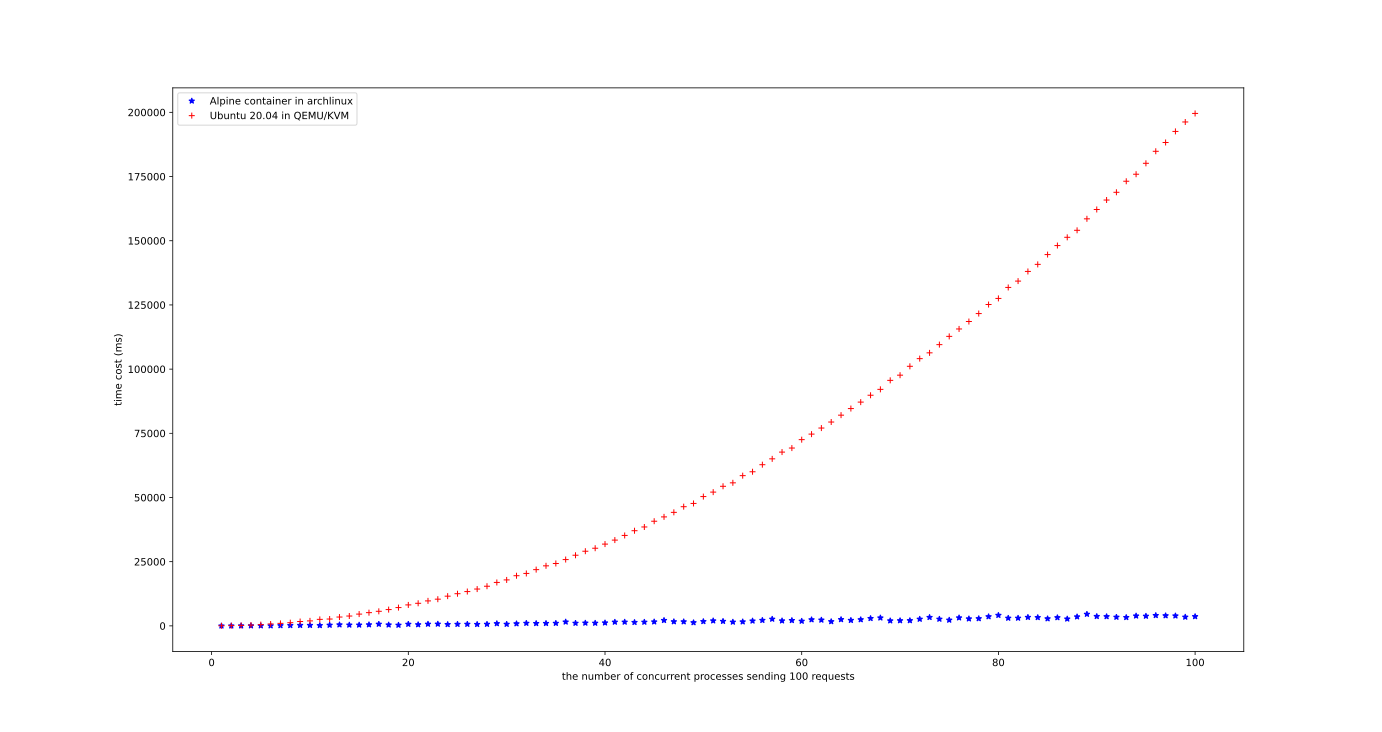
\includegraphics[width=\textwidth]{src/concurrent.png}
    \label{conc}
    \caption{Concurrent processes transporting time}
\end{figure}

\subsection{Throughput}
TBD\dots
\section{Conclusion}

We can see that the comparison results in virtual machine and container are
significantly indifferent order of time-consuming. There is no existence
of the gVisor's result because the gVisor was not able to launch the
IBM/FHIR server system, which is the target of our research.
We also expect that the gVisor might run faster significantly than the virtual
machine; however, our target cannot be launched successfully in
gVisor's sandbox.
We thought that there might have been some race condition bugs via JWE (JAVA Web
Engine) in gVisor, such that the gVisor did not do well in supporting all system calls.

And the time complexity of the virtual machine is significantly different from
the container. We propose a hypothesis of the time complexity of the virtual
machine, because there are more page fault events and the throughput limitation
of virtual machine device driver \cite{10.5555/1267569.1267570,7095802}.

The proposed scheme is nearly zero-overhead protection in the kernel, and
the policy is auto-generated and conformed in the build time. It could help
developers to deploy into a secure environment with no pain. This paper also
benchmarked the protection via virtual machine and our proposed scheme in
the container. It can be concluded that it is a good solution if we want
low latency and security.



\printbibliography[title=Reference]

\end{document}
